\begin{figure}[tbp]
\centering
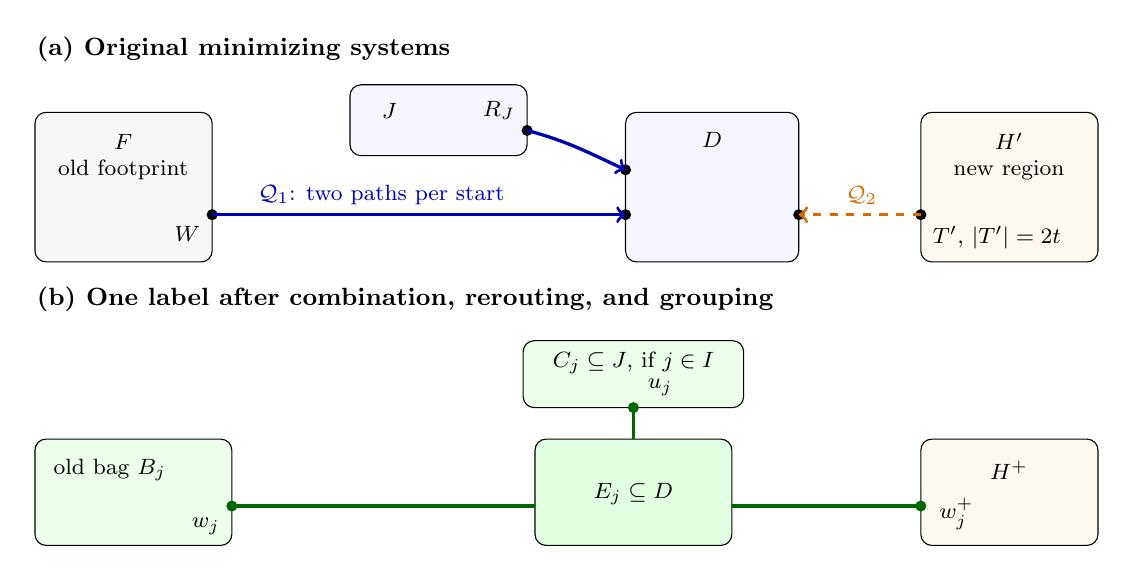
\begin{tikzpicture}[x=1cm,y=1cm,font=\footnotesize]
  \node[anchor=west,font=\small\bfseries] at (0,6.55)
    {(a) Original minimizing systems};
  \draw[rounded corners,fill=black!3] (0.1,3.85) rectangle (2.35,5.75);
  \node at (1.22,5.38) {\(F\)};
  \node at (1.22,5.02) {old footprint};
  \fill (2.35,4.45) circle (2pt);
  \node[below left] at (2.32,4.43) {\(W\)};

  \draw[rounded corners,fill=blue!4] (4.1,5.2) rectangle (6.35,6.1);
  \node at (4.6,5.77) {\(J\)};
  \fill (6.35,5.52) circle (2pt);
  \node[above left] at (6.32,5.53) {\(R_J\)};

  \draw[rounded corners,fill=blue!4] (7.6,3.85) rectangle (9.8,5.75);
  \node at (8.7,5.4) {\(D\)};
  \fill (7.6,4.45) circle (2pt);
  \fill (7.6,5.02) circle (2pt);
  \fill (9.8,4.45) circle (2pt);

  \draw[rounded corners,fill=orange!5] (11.35,3.85) rectangle (13.6,5.75);
  \node at (12.47,5.38) {\(H'\)};
  \node at (12.47,5.02) {new region};
  \fill (11.35,4.45) circle (2pt);
  \node[below right] at (11.38,4.43) {\(T'\), \(|T'|=2t\)};

  \draw[->,very thick,blue!70!black] (2.35,4.45) -- (7.6,4.45);
  \node[above,text=blue!70!black] at (4.5,4.45)
    {\(\mathcal Q_1\): two paths per start};
  \draw[->,very thick,blue!70!black]
    (6.35,5.52) to[out=-15,in=155] (7.6,5.02);
  \draw[->,very thick,dashed,orange!85!black]
    (11.35,4.45) -- (9.8,4.45);
  \node[above,text=orange!85!black] at (10.6,4.45)
    {\(\mathcal Q_2\)};

  \node[anchor=west,font=\small\bfseries] at (0,3.38)
    {(b) One label after combination, rerouting, and grouping};
  \draw[rounded corners,fill=green!8] (0.1,0.25) rectangle (2.6,1.6);
  \node at (1.05,1.21) {old bag \(B_j\)};
  \fill[green!40!black] (2.6,0.75) circle (2pt);
  \node[below left] at (2.57,0.72) {\(w_j\)};

  \draw[rounded corners,fill=green!12] (6.45,0.25) rectangle (8.95,1.6);
  \node at (7.7,0.9) {\(E_j\subseteq D\)};

  \draw[rounded corners,fill=green!8] (6.3,2.0) rectangle (9.1,2.85);
  \node at (7.7,2.57) {\(C_j\subseteq J\), if \(j\in I\)};
  \fill[green!40!black] (7.7,2.0) circle (2pt);
  \node[above right] at (7.76,2.03) {\(u_j\)};
  \draw[very thick,green!40!black] (7.7,2.0) -- (7.7,1.6);

  \draw[rounded corners,fill=orange!5] (11.35,0.25) rectangle (13.6,1.6);
  \node at (12.47,1.21) {\(H^+\)};
  \fill[green!40!black] (11.35,0.75) circle (2pt);
  \node[right] at (11.46,0.65) {\(w_j^+\)};
  \draw[very thick,green!40!black] (2.6,0.75) -- (6.45,0.75);
  \draw[very thick,green!40!black] (8.95,0.75) -- (11.35,0.75);
\end{tikzpicture}
\caption{A separability round, shown schematically.
The upper arrows represent families of paths; the two families may
intersect, and their entire vertex sets remain in the footprint.
Below, \(E_j\) joins label \(j\)'s path ends in \(D\).
The region \(H^+\) is obtained from \(H'\) by removing unused starts;
it meets the footprint exactly in the new tips \(W^+\).}
\label{fig:separability-round}
\end{figure}
